\chapter{Design}
The following chapter shall discuss the planning and design choices of the system. 



\newpage
\section{TODO Sequence Diagram}

\newpage
\section{Interface}

\begin{figure}[H]
    \centering
    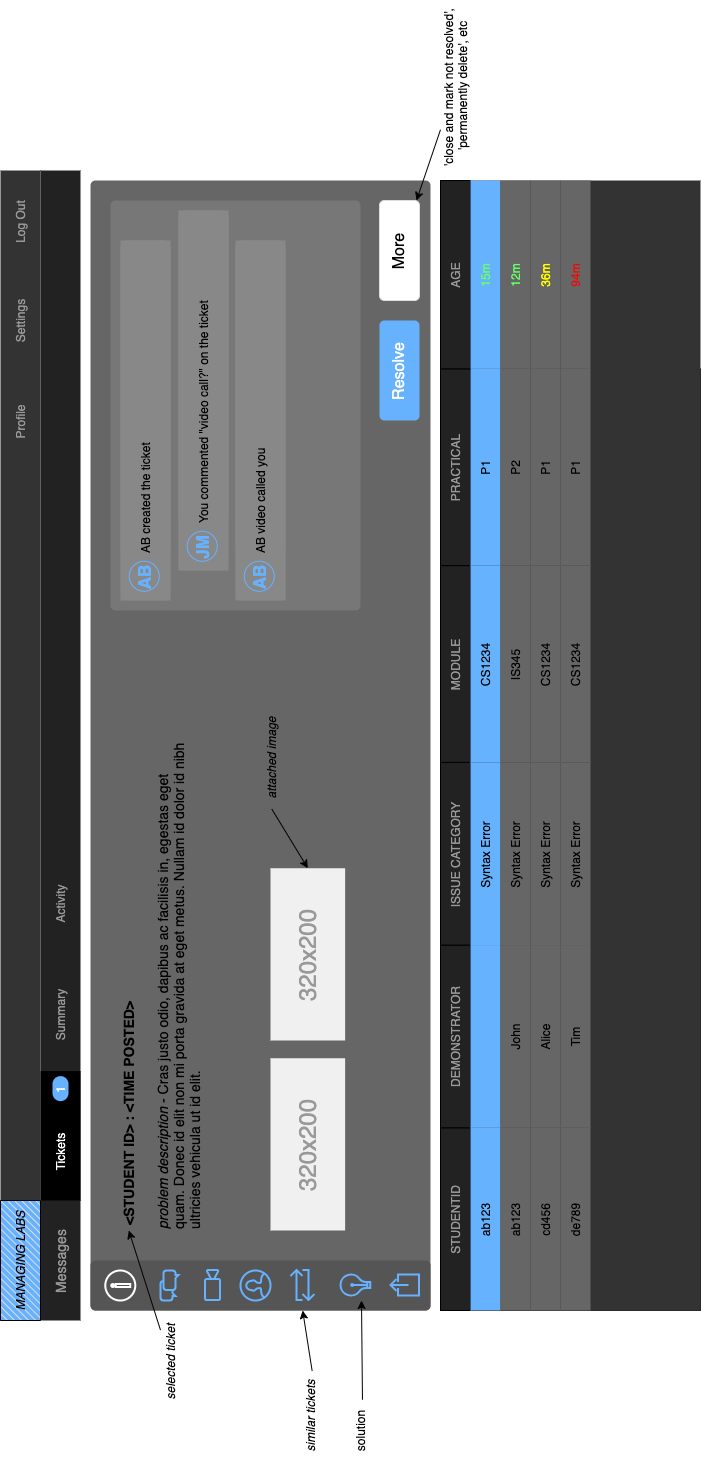
\includegraphics[width=0.6\textwidth]{7design/images/demoTickets.png}
    \caption{Simple design for the demo ticket viewing interface.}
    \label{fig:demoTickets}
\end{figure}

\section{Database}

\subsection{Entities, Attributes and Relationships}
We will now define a representation of the data in terms of entities, attributes and relationships between entities.

\subsubsection{Entities}

We represent the components of the systems as the following entities. 

\FloatBarrier
\begin{table}[H]
\centering
\begin{tabular}{ |l|c| } 
 \hline
 \textbf{Entity Set} & \textbf{Attributes}\\ 
 \hline
  user & \underline{userId}, name, password, loginStatus\\ 
 \hspace{6pt}user.student & \\ 
 \hspace{6pt}user.demonstrator & \\
 \hspace{12pt}user.demonstrator.labLead & \\
 sysAdmin & \underline{username}, password\\ 
 ticket & \underline{ticketId}, issueDescription,\\
 & practical, resolutionStatus \\
 attachment & \underline{attachmentId}, file, caption \\
 lab & \underline{labId}, openTime, closeTime\\
 solution & \underline{solutionId}, solutionDescription\\
 category & \underline{name} \\
 module & \underline{moduleCode} \\
 \hline
\end{tabular}
\caption{Table of entities and associated attributes.}
\end{table}
\FloatBarrier

Primary keys are denoted as \underline{underlined}. Foreign keys are denoted in \textit{italics}.

Note that \textbf{user.student} and \textbf{user.demonstrator} are disjoint specialisations of the entity set \textbf{user} - a user is always a student or demonstrator (or specialisation of demonstrator). \textbf{user.demonstrator.labLead} is a further specialisation of \textbf{user.demonstrator}, not disjoint. 

\subsubsection{Relationships}
We shall now define the relationships between entities and the constraints on them. 

\FloatBarrier
\begin{table}[H]
\centering
\begin{tabular}{ |c|c|c|c| } 
 \hline
 \textbf{Relationship} & \textbf{Entities} & \textbf{Participation} & \textbf{Cardinality}\\ 
 \hline
 $r$ & $e_1$, $e_2$ & total, partial & M-1 \\
 \hline
\end{tabular}
\end{table}
\FloatBarrier 

We denote many as M, one as 1 such that one to many relationship would be denoted 1-M. Note that for a relationship $r$ that is many (in $e_1$) to one (in $e_2$) and has total participation from $e_1$ but partial from $e_2$ then the row in the table is written as above. Participation will be listed in order that entities are written.

\FloatBarrier
\begin{table}[htbp]
\centering
\resizebox{\columnwidth}{!}{\begin{tabular}{ |c|c|c|c|c| } 
 \hline
 \textbf{Relationship} & \textbf{Relationship Attributes} & \textbf{Entity Sets} & \textbf{Participation} & \textbf{Cardinality}\\ 
 \hline
 creates & creation\_timestamp & user.student, ticket & partial, total & 1-M \\
 assignedTo & demAssigned\_timestamp & user.demonstrator, ticket & partial, partial & 1-M\\
 writes & demSolved\_timestamp & user.demonstrator, solution & partial, total & M-M\\
 leads & & user.demonstrator.labLead, lab & partial, total & 1-M\\
 hasAttachment & ticket\_attach\_timestamp & ticket, attachment & partial, partial & 1-M\\
 hasAttachment & solution\_attach\_timestamp & solution, attachment & partial, partial & 1-M\\
 postedIn &  & ticket, lab & total, partial & M-1\\
 hasTicketCat & & ticket, category & total, partial & M-M\\
 hasSolutionCat & & solution, category & total, partial & M-M\\
 demonstratesIn & & user.demonstrator, lab & partial, total & M-M\\
 enrolledInMod && user.student, module & total, partial & M-M\\
 demonstratesInMod && user.demonstrator, module & partial, partial & M-M\\
 leadsMod && user.ladLead, module & partial, partial & 1-M\\
 toDoWith && ticket, module & total, partial & M-1\\
 \hline
\end{tabular}}
\caption{Table showing entities, relationships between, relationship attributes, participation and cardinality.}
\end{table}
\FloatBarrier

\subsubsection{Entity Relationship Diagram}

\begin{figure}[H]
    \centering
    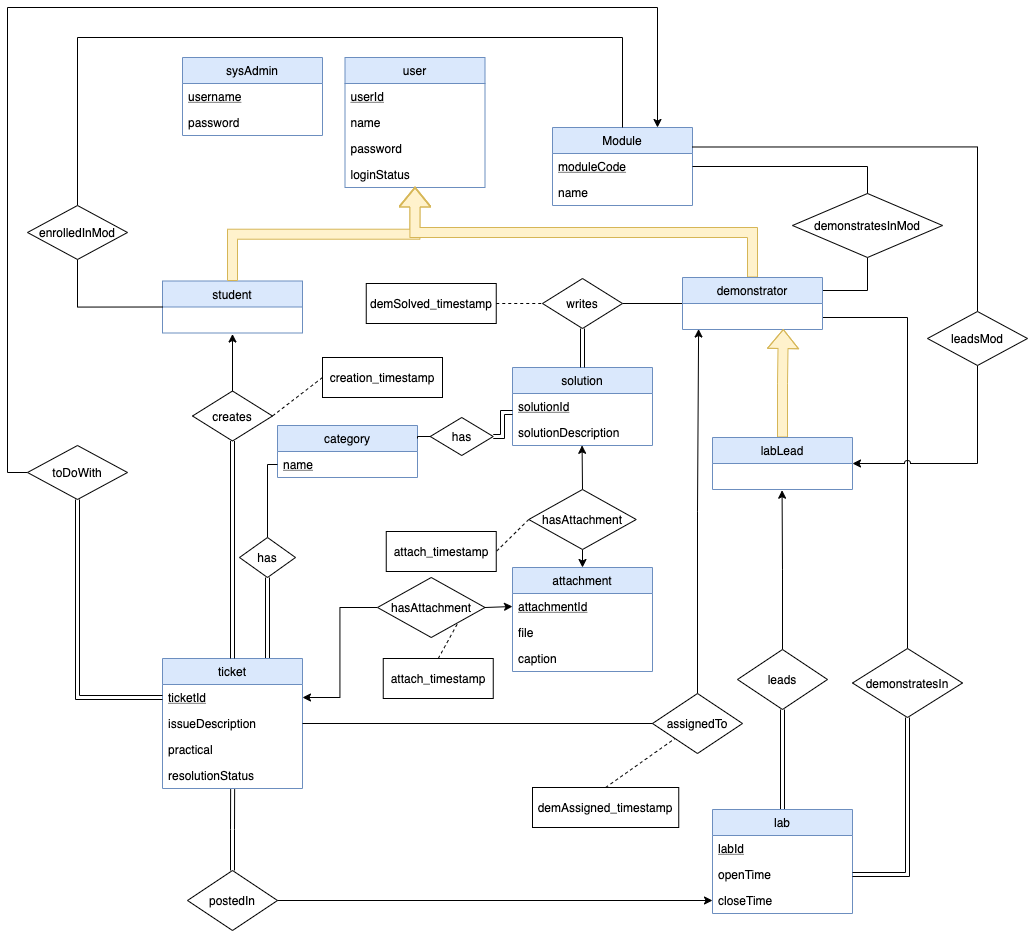
\includegraphics[width=\textwidth]{7design/images/ER.png}
    \caption{\gls{er} diagram for the system.}
    \label{fig:ER}
\end{figure}

\subsubsection{Relational Schema}
The first task is to translate the given E-R model into corresponding database schema below.\\

\noindent student - \underline{userId}, name, password, loginStatus, enrolledModules \\
demonstrator - \underline{userId}, name, password, loginStatus, demonstratedModules \\
labLead - \underline{userId}, name, password, loginStatus, demonstratedModules, ledModules \\
sysAdmin - \underline{username}, password \\
ticket - \underline{ticketId}, issueDescription, module, practical, resolutionStatus, \textit{student.userId}, creation\_timestamp, \textit{demonstrator.userId}, demAssigned\_timestamp, \textit{labId} \\
category - \underline{name} \\
solution - \underline{solutionId}, solutionDescription\\
attachment - \underline{attachmentId}, file, caption, \textit{ticketId}, ticket\_attach\_timestamp, \textit{solutionId}, solution\_attach\_timestamp\\
lab - \underline{labId}, openTime, closeTime, \textit{labLead.userId}\\
writes - \underline{\textit{demonstrator.userId}}, \underline{\textit{solutionId}}, demSolved\_timestamp\\
hasTicketCat - \underline{\textit{tickedId}}, \underline{\textit{name}}\\
hasSolutionCat - \underline{\textit{solutionId}}, \underline{\textit{name}}\\
demonstratesIn - \underline{\textit{demonstrator.userId}}, \underline{\textit{labId}}\\
module - \underline{moduleCode}, name, \textit{labLead.userId}\\
enrolledInMod - \underline{\textit{student.userId}}, \underline{\textit{moduleCode}}\\
demonstratesInMod - \underline{\textit{demonstrator.userId}}, \underline{\textit{moduleCode}}\\

\subsubsection{Relational Schema Diagram}

\begin{figure}[H]
    \centering
    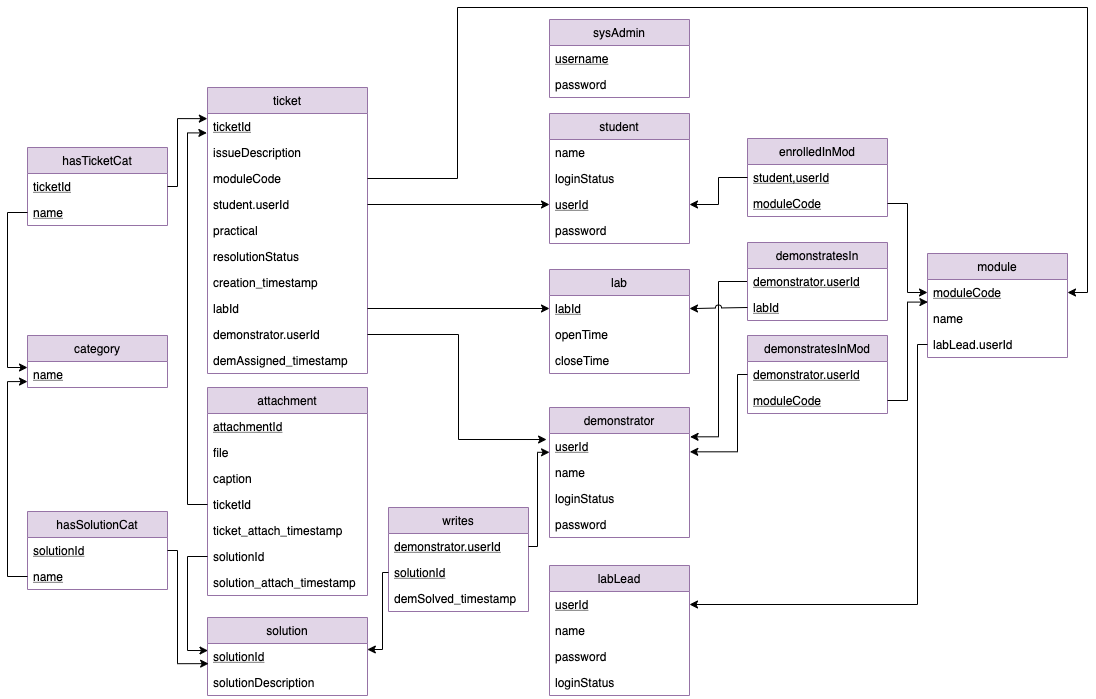
\includegraphics[width=\textwidth]{7design/images/relationalSchema.png}
    \caption{Relational schema diagram for the system.}
    \label{fig:relationalschema}
\end{figure}

\subsubsection{Attribute Types}
A data type must be specified for each attribute. Table \ref{table:atypetable} below shows the attribute type for each attribute, as well as it's original, parent relational table - in other words, we do not repeat the attributes that appear as foreign keys in tables.

\begin{table}[H]
\centering
\begin{tabular}{| c | c | c |}
\hline
 Relational Table & Attribute & Attribute Type \\ 
 \hline
  category & name & ? \\
  \hline
  ticket & ticketId & \\
  & issueDescription & \\
  & practial & \\
  & resolutionStatus & \\
  & creation\_timestamp & \\
  &  demAssigned\_timestamp & \\
  \hline 
  attachment & attachmentId & \\
  & file & \\
  & caption & \\
  & ticket\_attach\_timestamp & \\
  & solution\_attach\_timestamp & \\
  \hline
  solution & solutionId & \\
  & solutionDescription & \\
  \hline
  writes & demSolved\_timestamp & \\
  \hline
  sysAdmin & username & \\
  & password & \\
  \hline
  student & name & \\
  & loginStatus & \\
  & userId & \\
  & password & \\
  \hline
  lab & labId & \\
  & openTime & \\
  & closeTime & \\
  \hline
  demonstrator & userId & \\
  & name & \\
  & loginStatus & \\
  & password & \\
  \hline
  labLead & userId & \\
  & name & \\
  & password &  \\
  & loginStatus & \\
  \hline
  module & moduleCode & \\
  & name & \\
 \hline
 
 \hline
\end{tabular}
\caption{Table describing the data types for attributes, showing the parent relational table.}
\label{table:atypetable}
\end{table}

The Government Data Standards Catalogue\cite{dataStandards} was referenced for data types of name, address line, number, email, account number. The logical extension was to apply the name data type to supplier name, genre\_name, author, publisher. For country.name, we also allow 70 characters - even though this is excessive, we allow for the possible entry of countries with longer names. The attributes `customer\_address\_country' and `deliv\_add\_country' are stored using a 3 digit code, defined by the ISO 3166-1 standard\cite{iso}. Although the Government Data Standards Catalogue had a reference for postcodes of VARCHAR(8), it was for UK postcodes - international postcodes/area codes could be longer and so the data type VARCHAR(35) was chosen to keep it in line with the address line attributes.

For the rating attribute, we assume that rating is given and stored in 1 d.p. increments from 0 to 5. We assume that no book that the store buys or sells will cost more than £9999.99 - assuming the currency is in GBP. Another assumption we make is that editions can come in 0.1 increments, and that no book has edition over `999.99'. The data type INT was selected for IDs, this is because we do not know the scale or projected scale of the store and so can store a large number of values - it also allows us to implement automatic incrementing for the ID attributes in SQL. The value MEDIUMINT was considered for IDs, to improve scan time at the cost of possible number of values, however because I was unsure of the scale of the bookstore so I erred on the side of caution with INT. We should note the fact that ISBNs cannot be used as, in the ER diagram given, the relationship between book and edition is not one to one - implying that different editions and types of a book will have one ID. Note that the different IDs could be formatted in different ways. The attribute type was store as CHAR(9) - this is because the type must be one of `audiobook', `hardcover' or `paperback', each being nine characters long. 
